\chapter{Data Collection}
\label{cha:data_collection}

In this chapter, we provide a comprehensive account of the data collection process
that underpins our experiments. We detail the key steps involved in designing, implementing,
and refining our methodology, with a particular focus on the construction and optimization
of the prompts used to interact with the Large Language Model (LLM).

We begin by presenting the core prompts utilized in our study, describing their
specific applications within each experimental setup. Following this, we outline
the rationale behind our prompt design decisions, grounding our choices in relevant
literature and highlighting key findings from previous research that informed our
approach.

Finally, we introduce the structure of our experimental evaluations, including the
generation of specialized heatmaps designed to illustrate the agent's uncertainty
in action selection. These visualizations provide valuable insights into the
model's decision-making process, highlighting both its generative strengths and areas
for further refinement.

\section{Prompts}
\label{sec:prompts}

This section provides a general overview of the prompts used in our experiments,
while the following one (Section \ref{sec:prompt_creation_choices}) will detail the
specific choices behind each specific part of them. The prompts were designed to
be concise yet comprehensive, ensuring that they effectively elicited the desired
responses from the model.

In the next subsections, we will present two core prompts that formed the
foundation of our experiments. These prompts were specifically designed to assess
the model's ability to generate optimal actions (one at the time) in our two main
tasks: picking up and delivering a parcel.

This section provides a general overview of the prompts used in our experiments.
While the subsequent section (Section \ref{sec:prompt_creation_choices}) delves into
the specific design choices behind each component, here we present the
fundamental structure and intent of the core prompts.

Our prompts were designed to be both concise and comprehensive, ensuring they effectively
guided the model in generating appropriate next-step actions. The core idea was
to elicit responses that incrementally moved the agent toward its objective, either
picking up or delivering a parcel, while minimizing ambiguity in the
instructions.

The two primary prompts used in our study are:
\begin{itemize}
  \item Pickup prompt: guiding the agent to retrieve a parcel from a specified
    location;

  \item Delivery prompt: prompting the agent to transport the parcel to its
    designated drop-off point.
\end{itemize}

Each prompt was carefully structured to provide relevant contextual information
while avoiding unnecessary complexity that could dilute the model's focus.

\subsection{Pickup prompt}
\label{sub:pickup_prompt}

The Pickup prompt (Listing \ref{lst:pickup_prompt}) was used to evaluate the model's
ability to generate actions in the \emph{pickup} scenario. In this setup, the
agent was tasked with picking up a parcel from a specific location on the map. The
prompt provided the agent with the raw map information, including the map
dimensions, the location of the parcel, and the agent's current position.

The model was then asked to determine the optimal next action that would bring
the agent one step closer to the parcel.

\begin{codewindow}
  [Text] \lstset{style=promptstyle, language=prompt, caption={Pickup prompt used in the experiments},
  label={lst:pickup_prompt}} \begin{lstlisting}
You are a delivery agent in a web-based delivery game where the map is a matrix
I am going to give you the raw information I receive from the server and the possible actions.
Map width: {width}
Map height: {height}
Tiles are arranged as {height} rows in {width} columns:
{tiles}
The parcel you need to take is in the spot ({parcelX}, {parcelY}).
You are on the spot ({agentX}, {agentY}).
The actions you can do ONLY if the next tile is available are:
U) move up
D) move down
L) move left
R) move right
T) take the parcel that is in your tile
S) ship a parcel (you must be in a delivery tile)

Your final goal is to go to a tile with the parcel and (T)ake it, I need the best action that will get you there.
Don't explain the reasoning and don't add any comment, just provide the action's letter.
What is your next action?
\end{lstlisting}
\end{codewindow}

\subsection{Deliver prompt}
\label{sub:deliver_prompt}

The Delivery Prompt (Listing \ref{lst:deliver_prompt}) was structured to
evaluate the model's ability to navigate toward a designated drop-off location. Unlike
the Pickup Prompt, where the parcel's position was explicitly provided, the delivery
prompt required the LLM to infer the delivery destination from the map description.
The model was then asked to determine the best next action to move toward the
inferred delivery location.

\begin{codewindow}
  [Text] \lstset{style=promptstyle, language=prompt, caption={Deliver prompt used in the experiments},
  label={lst:deliver_prompt}} \begin{lstlisting}
You are a delivery agent in a web-based delivery game where the map is a matrix
I am going to give you the raw information I receive from the server and the possible actions.
Map width: {width}
Map height: {height}
Tiles are arranged as {height} rows in {width} columns:
{tiles}
You are on the spot ({agentX}, {agentY}).
The actions you can do are:
U) move up
D) move down
L) move left
R) move right
T) take the parcel that is in your tile
S) ship a parcel (you must be in a delivery tile)

You have a parcel to ship, your final goal is to go to the delivery zone (delivery = true) and (S)hip the parcel, I need the best action that will get you there.
Don't explain the reasoning and don't add any comment, just provide the action's letter.
What is your next action?
\end{lstlisting}
\end{codewindow}

\section{Prompt Creation Choices}
\label{sec:prompt_creation_choices}

This section outlines the key considerations that guided the construction of our
prompts (commonly referred to as Prompt Engineering). We describe the reasoning behind
specific design choices, following the sequence in which they appear in the
prompt. For clarity, we use the Pickup Prompt (Listing \ref{lst:pickup_prompt})
as a reference.

\subsection{Role Prompting}
Assigning specific roles or personas to Large Language Models (LLMs) within
prompts, known as ``role prompting," has been shown to enhance their performance
on various tasks. This technique involves instructing the model to assume a
particular identity, such as a ``math professor" or ``geographer," to guide its
responses more effectively. The concept of role prompting has been explored in several
studies.

For instance, the paper `Better Zero-Shot Reasoning with Role-Play Prompting' by
Kong et al. \cite{kong2024betterzeroshotreasoningroleplay} demonstrated that strategically
designed role-play prompts can significantly improve LLMs' reasoning abilities
across diverse benchmarks.

Similarly, `Role-Play Zero-Shot Prompting with Large Language Models for Open-Domain
Human-Machine Conversation' by Njifenjou et al.
\cite{njifenjou2024roleplayzeroshotpromptinglarge} investigated the use of role-play
prompts to enhance conversational agents' performance without additional fine-tuning.

In our experiments, we employed role prompting to encourage the model to adopt
the persona of a \emph{delivery agent}, thereby focusing its attention on the
task at hand. By framing the prompts in this manner, we aimed to guide the model's
responses towards generating coherent and contextually relevant actions.

\subsection{Map Encoding to Reduce Attention Sparsity}

One of our primary concerns was that the map included in the prompt might take up
too much space, which could lead to an excessively sparse distribution of
attention. This could result in the model not properly focusing on crucial aspects
of the input. At the same time, we wanted to maintain a minimal and flexible approach
to map handling. Our goal was to ensure that the system would continue
functioning even if the format of the map-providing function were to change
unexpectedly. As discussed in Section \ref{sub:our_task}, this design decision
was made to simulate an unpredictable and rapidly changing environment.

To address this concern, we first aimed to understand how the model processed map-related
information. Ideally, we would have examined the models's attention scores directly,
but unfortunately, OpenAIss API does not provide access to these scores. As a
result, we had to rely on a qualitative analysis instead. To achieve this, we leveraged
BERT, another Transformer-based architecture, to visualize attention patterns in
our original prompt. The results revealed that a significant portion of the
models's attention was focused on tokens related to JSON syntax rather than the
meaningful content of the prompt itself. This suggested that structural elements,
rather than semantic information, were drawing a disproportionate amount of attention.

Based on this observation, we attempted to reduce the presence of JSON syntax
within the prompt while preserving the essential information. We then repeated the
same attention analysis using this modified version. The results showed a
notable shift in the distribution of attention, even if the two prompts contained
virtually the same information. Specifically, when we examined the tokens receiving
the highest attention — excluding punctuation, as well as the special starting
and ending tokens — we found that in the original prompt, only 23 out of the top
50 tokens were meaningful words. In contrast, in the revised prompt, this number
increased to 31 out of 50, indicating a more focused attention on relevant content.

For this test, we used an older version of the ``Pickup prompt", which is
explained in detail in Section \ref{sec:second_approach}, with a small 2x5 map.
As demonstrated in Table \ref{tab:prompt_comparison}, the revised version of the
prompt not only contained more words in the top 50 tokens, but also explicitly
included the term \textbf{pickup}, which is the key focus of our task. Notably,
this term was entirely absent from the top attention-receiving tokens in the
initial prompt.

\begin{table}[ht]
  \centering
  \begin{tabular}{|c|c|}
    \hline
    \textbf{Old Prompt} & \textbf{New Prompt} \\
    \hline
    game                & game                \\
    reasoning           & parcel              \\
    parcel              & reasoning           \\
    parcel              & i                   \\
    score               & actions             \\
    response            & you                 \\
    parcel              & if                  \\
    tile                & parcel              \\
    i                   & moves               \\
    if                  & height              \\
    you                 & width               \\
    response            & score               \\
    loop                & ship                \\
    comment             & tile                \\
    information         & loop                \\
    actions             & information         \\
    and                 & choosing            \\
    ship                & you                 \\
    and                 & \textbf{pickup}     \\
    server              & and                 \\
    you                 & you                 \\
    choosing            & parcel              \\
    using               & and                 \\
                        & server              \\
                        & information         \\
                        & and                 \\
                        & ship                \\
                        & explain             \\
                        & using               \\
                        & reward              \\
                        & name                \\
    \hline
  \end{tabular}
  \caption{Comparison of Old and New Prompts}
  \label{tab:prompt_comparison}
\end{table}

To further analyze the impact of this change, we collected attention scores from
both the old and new prompt versions. We then removed the tokens corresponding to
the map representation in both prompts and plotted the difference between the attention
in the remaining common 264 tokens. The resulting visualization is presented in
Figure \ref{fig:difference} as
$old\_prompt\_attention - new\_prompt\_attentio n$. Interpreting this figure is not
entirely straightforward, and we acknowledge that it is unclear to what extent
this analysis can serve as a direct proxy for a GPT-based model. However, one
noticeable trend is that the diagonal elements exhibit a lower overall attention
intensity (indicated by the presence of purple and dark blue regions). Meanwhile,
most of the remaining areas show a delta close to zero (represented in aqua blue),
suggesting that the changes we introduced led to a redistribution of attention without
introducing excessive noise or unintended biases. While this number does not
have a direct interpretative meaning, for completeness, we note that the total
sum of the difference matrix is about $- 15.34476$, indicating more attention in
the new version of the prompt.

\begin{figure}[ht!]
  \centering
  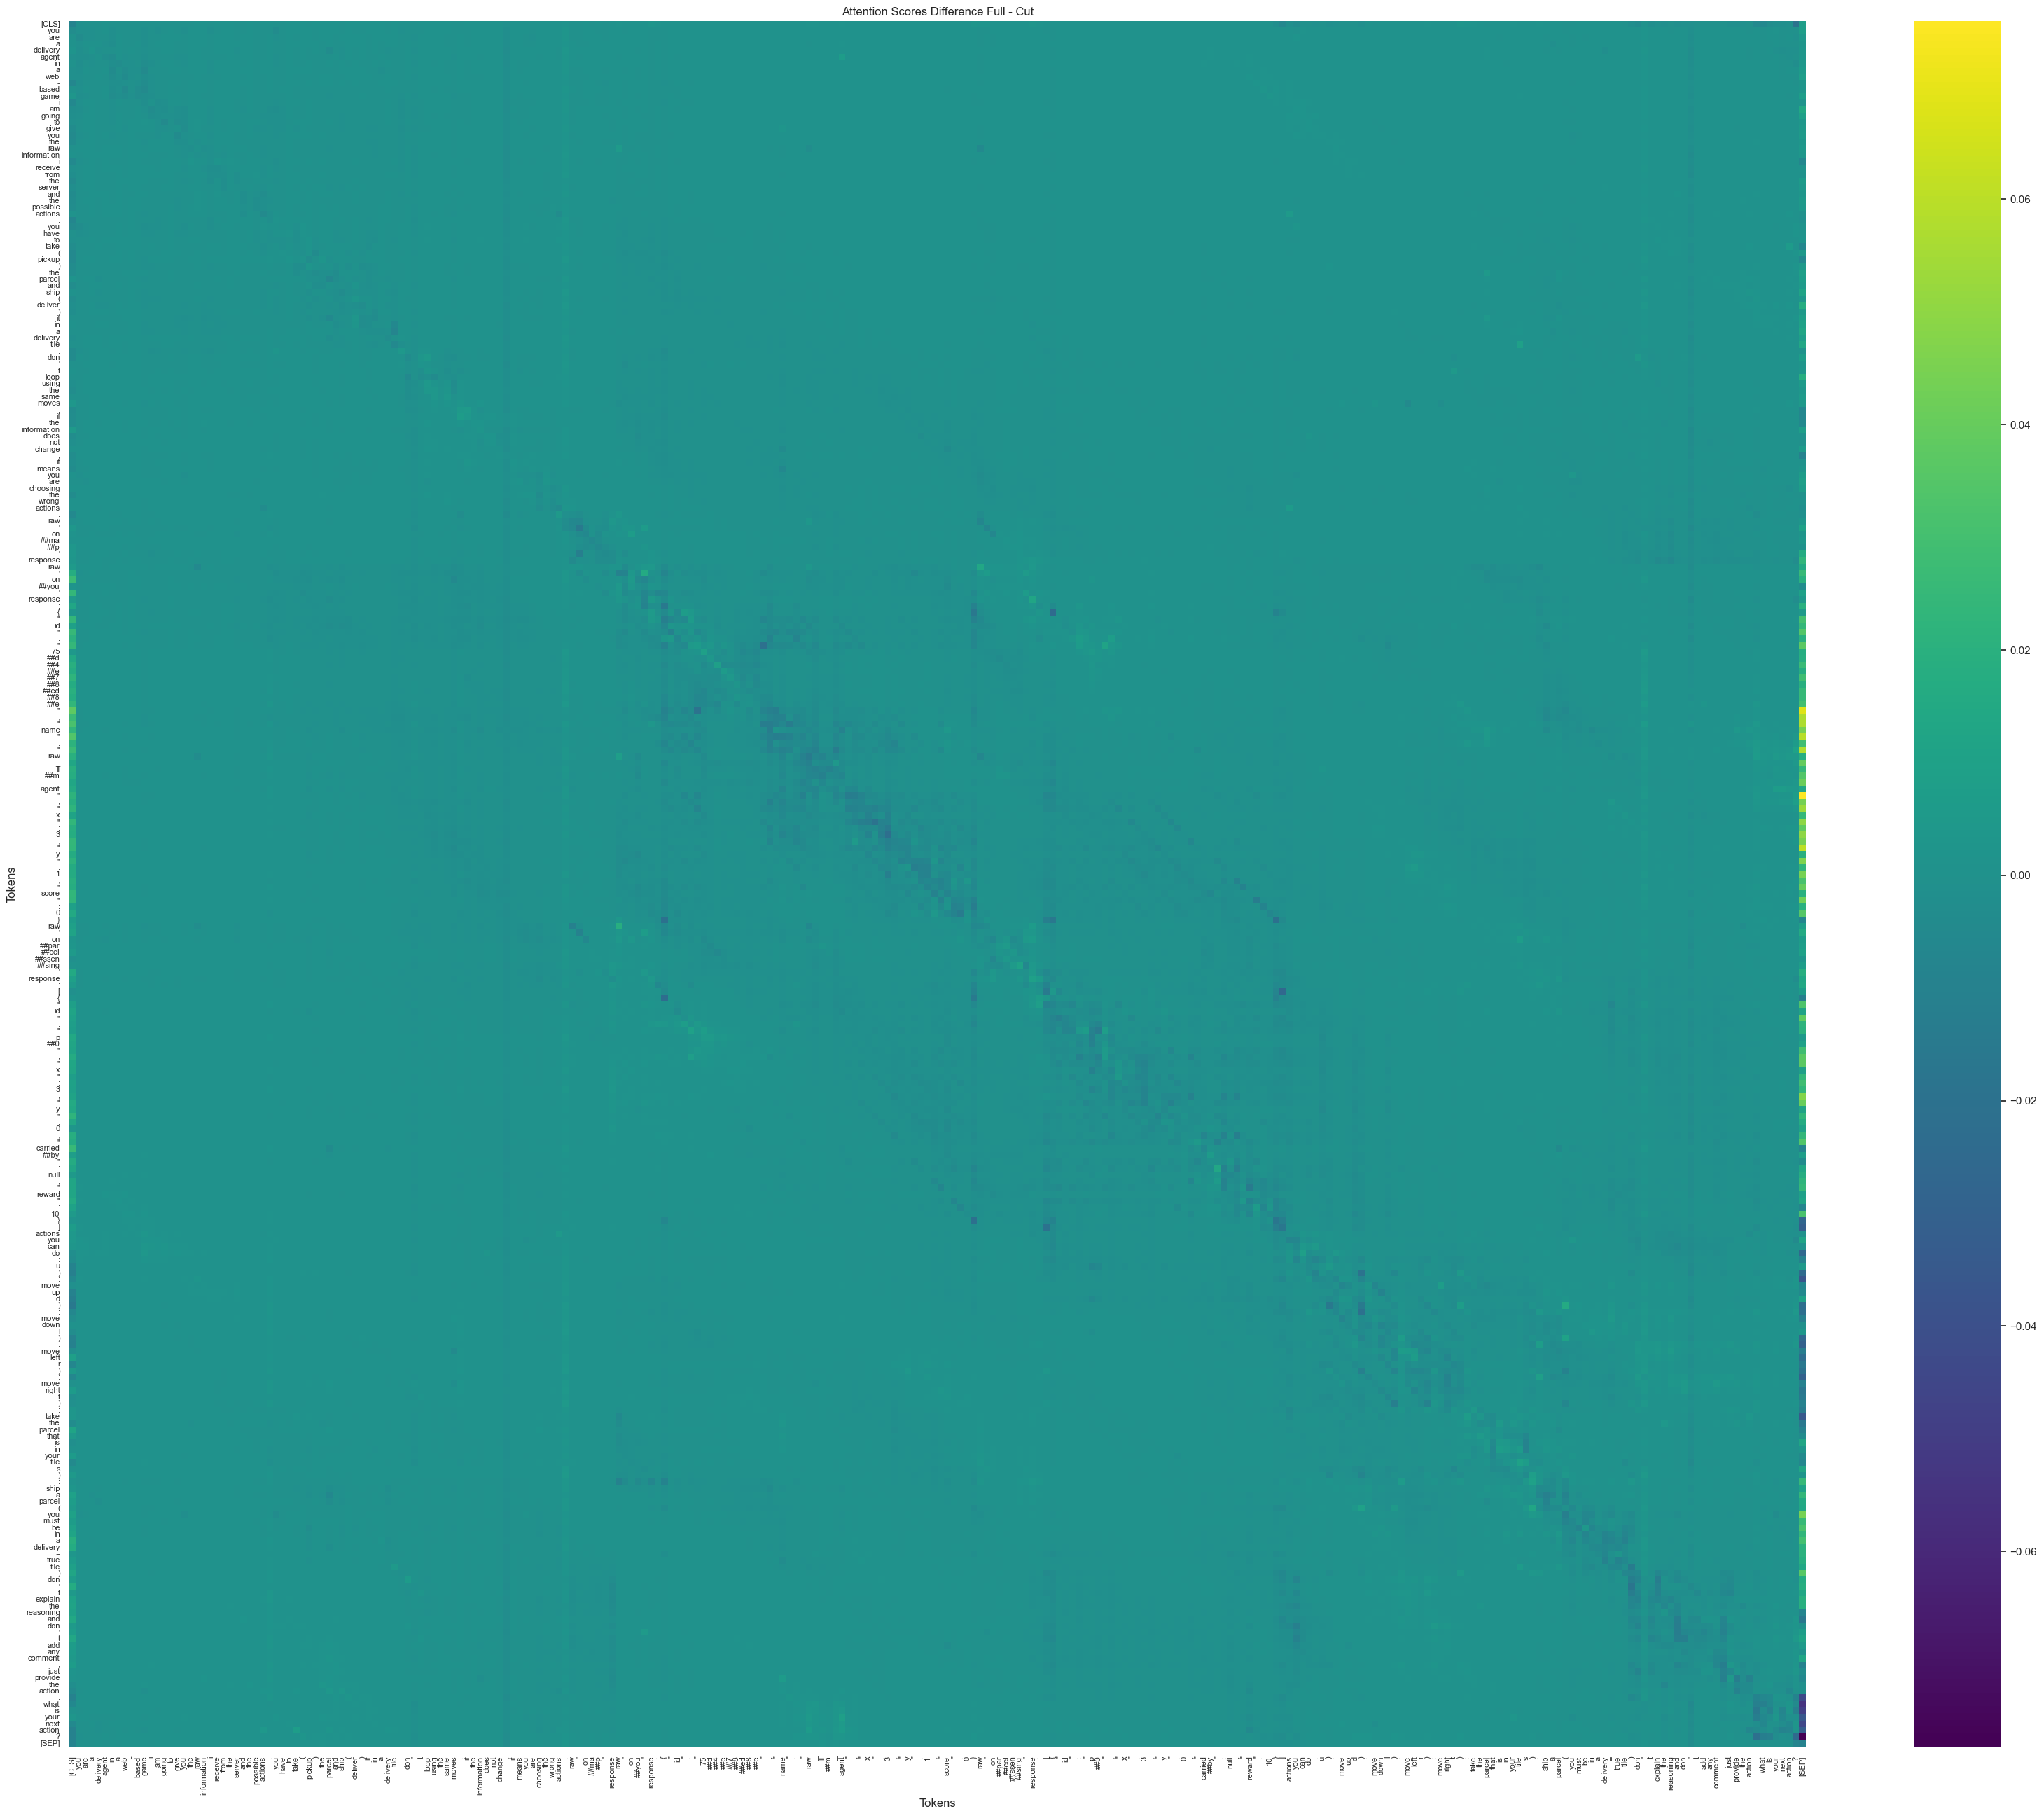
\includegraphics[width=0.8\textwidth]{images/data_collection/difference.png}
  \caption{Attention Difference between Old and New Prompts 264 common tokens. Full
  resolution available in the repository \cite{projectrepo}.}
  \label{fig:difference}
\end{figure}

\subsubsection{Emerging behavior: encoded question decoded answer}

Another strategy we explored to reduce the space occupied by the map in the prompt
was to encode it. Our goal was to compress the map representation while ensuring
that the model could still understand the relevant information.

A relevant study on this topic is presented in the paper `LLMs Can Understand Encrypted
Prompt: Towards Privacy-Computing Friendly Transformers" \cite{liu2023llmsunderstandencryptedprompt}.
The authors of this paper aimed to preserve user privacy by encrypting prompts
before sending them to a language model. Their findings demonstrated that the model
was able to comprehend and respond appropriately to encrypted prompts. This
suggested that LLMs possess an inherent ability to process encoded text
meaningfully.

Inspired by these results, we conducted an experiment to determine whether a similar
encoding approach could be used to reduce the space occupied by the map while preserving
its usability within the prompt. Specifically, we investigated whether the model
could still interpret a compressed version of the map if it were encoded.

\vspace{5mm}
\begin{figure}[ht!]
  \centering
  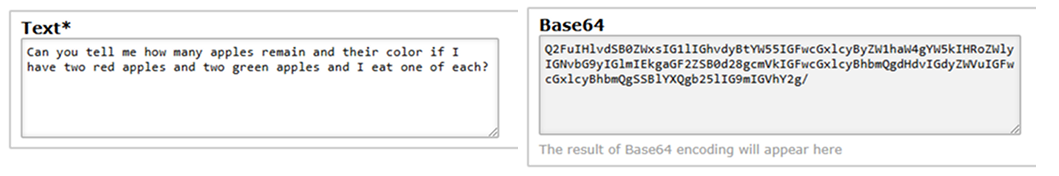
\includegraphics[width=0.98\textwidth]{images/data_collection/texttob64.png}
  \caption{Base64 encoding of a sample text}
  {\emph{Source: base64.guru}\footnotemark} \label{fig:texttob64}
\end{figure}
\footnotetext{\url{https://base64.guru/converter/encode/text}}
\vspace{5mm}

To validate this, we first examined the model's ability to process encoded prompts
by testing a simple case. As shown in Figure \ref{fig:b64gpt}, the model successfully
understood the meaning of the question ``Can you tell me how many apples remain and
their color if I have two red apples and two green apples and I eat one of each?"
even when the entire prompt was encoded in BASE64 (see Figure
\ref{fig:texttob64}). Notably, the model did not generate a decoding function before
answering. Instead, it directly processed the encoded prompt and returned a response
in plain English, demonstrating its ability to work with BASE64-encoded text.

\begin{figure}[ht!]
  \centering
  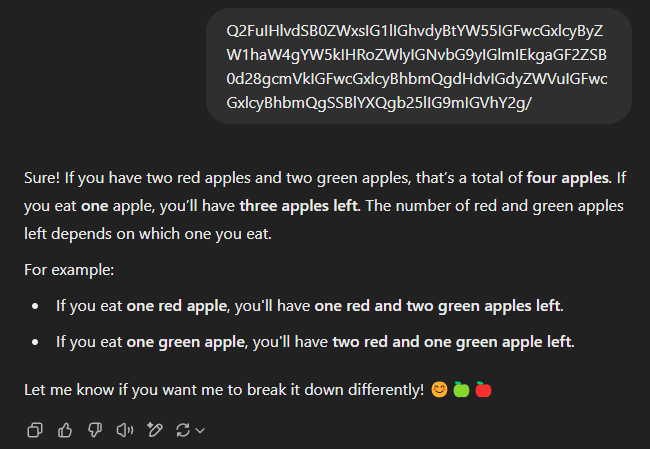
\includegraphics[width=0.66\textwidth]{images/data_collection/b64gpt.png}
  \caption{GPT-4o-mini response to a BASE64-encoded question}
  {\emph{Source: GPT-4o-mini via OpenAI web interface}} \label{fig:b64gpt}
\end{figure}

Encouraged by these results, we attempted to apply a similar encoding strategy
to the map representation while also aiming to reduce the number of characters
in the prompt. Our hypothesis was that reducing the character count would also reduce
the number of tokens, thereby improving attention efficiency.

To test this, we implemented a two-step encoding process in Python, as outlined
in Listing \ref{lst:double_enc}:
\begin{enumerate}
  \item First, we compressed the map using the \texttt{zlib} library and its Deflate
    algorithm \footnote{\url{https://en.wikipedia.org/wiki/Deflate}} to minimize
    its size;

  \item Next, we encoded the compressed output in BASE64 \footnote{\url{https://en.wikipedia.org/wiki/Base64}}
    using the \texttt{base64} library;

  \item Finally, we inserted this doubly encoded map into the prompt.
\end{enumerate}

\vspace{5mm}
\begin{codewindow}
  [Python Code] \lstset{style=pythonstyle, language=Python, caption={Example of double encoding algorithm},
  label={lst:double_enc}} \begin{lstlisting}
[...]

input_string = MAP
compressed_data = zlib.compress(input_string.encode('utf-8'))
compressed_base64 = base64.b64encode(compressed_data).decode('utf-8')

[...]
\end{lstlisting}
\end{codewindow}
\vspace{5mm}

While this method did succeed in reducing the number of characters by $\sim 65\%$,
the results were not as expected in terms of model comprehension. Unlike the case
of simple BASE64 encoding, the LLM was no longer able to interpret the prompt
correctly. Instead, its responses typically fell into one of two categories:
\begin{itemize}
  \item The model would explicitly state that it recognized the input as an encrypted
    message and generate something similar to ``It seems you've provided a compressed
    string or encoded data. Could you clarify how you'd like to use or process
    this? If it's encoded text, I can try decoding it for you.";

  \item Alternatively, if instructed with the encryption method used on the text,
    the model would generate a Python function to decode the input before attempting
    to process it. Such a function would have been executed ``under the hood" to
    decrypt the message before processing.
\end{itemize}

Furthermore, although our approach successfully reduced the total number of characters
in the prompt, it did not achieve our ultimate objective.

We then tried only using the BASE64 encoding, but the number of character actually
increased rather than decreased as well as the number of tokens that increased even
more in percentage. This is because tokenization in LLMs is based on common
character sequences rather than individual characters. Encoding the map disrupted
these common patterns, leading to a tokenization process that resulted in a
higher overall token count. Consequently, the intended effect of reducing
attention sparsity was not achieved, as illustrated in Figure \ref{fig:lesscharmoretokens}.

\vspace{5mm}
\begin{figure}[ht!]
  \centering
  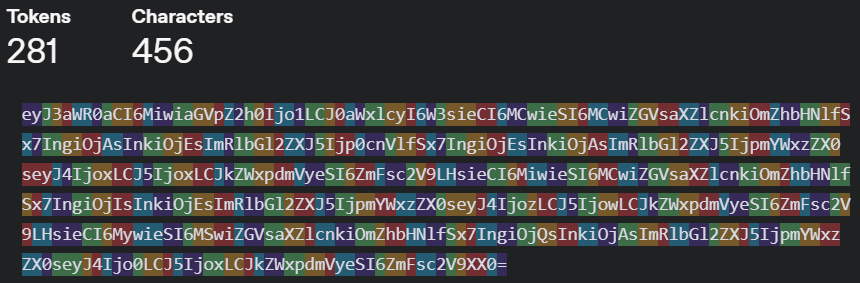
\includegraphics[width=0.66\textwidth]{
    images/data_collection/lesscharmoretokens.png
  }
  \caption{Tokenization of a BASE64-encoded text}
  {\emph{Source: GPT-4o tokenizer via OpenAI web interface}} \label{fig:lesscharmoretokens}
\end{figure}
\vspace{5mm}

In summary, while encoding techniques like BASE64 alone might be useful for preserving
meaning in certain contexts, our specific approach of compressing and encoding
the map did not lead to the desired efficiency gains. Instead, it introduced
additional computational overhead for the model, ultimately making this approach
ineffective for our purposes.

\subsection{Emerging behavior: math capabilities}

We also investigated the impact of including action-related information, such as
explicitly stating ``Going up increases your X position by 1" for every movement
action. It initially seemed like a promising way to guide the model's reasoning.
However, this conflicted with our overarching goal of keeping the system adaptable
rather than grounding it in a fixed environmental structure. Despite this, we proceeded
with the experiment to assess its impact.

Interestingly, we observed that the model's performance in navigation tasks was
unexpectedly strong, even to the point of raising concerns about potential shortcuts.
To further investigate, we conducted a follow-up test in which we entirely removed
the map from the prompt. As result, the model still produced correct answers by seemingly
ignoring any extraneous details and reducing the problem to simple arithmetic.
It recognized that if the starting position was \texttt{(4,2)} and the goal was at
\texttt{(0,0)}, the necessary movement was simply decreasing \texttt{X} by 4 and
\texttt{Y} by 2. This behavior demonstrated that the model could abstract away the
spatial representation and ``cheating'' by operating purely on mathematical reasoning.

This finding aligns with existing research on the emergent mathematical reasoning
capabilities of large language models. For example, Wei et al. highlight how
LLMs exhibit "emergent abilities", capabilities that do not appear in smaller models
but spontaneously manifest as model scale increases \cite{wei2022emergentabilitieslargelanguage}.
Among these abilities, arithmetic and mathematical reasoning are particularly notable,
suggesting that LLMs can generalize numerical patterns without explicit training
for such tasks. Our experiment provides anecdotal evidence supporting this:
rather than relying on the environmental constraints provided in the prompt, the
model instinctively leveraged its inherent mathematical capabilities to deduce the
necessary movements. Ultimately, given this behavior, we abandoned the idea of
including the results of the actions in the prompt.

\subsection{Question Structure}

A summarized example of a prompt used in the paper \emph{Robots That Ask For
Help: Uncertainty Alignment for Large Language Model Planners}
\cite{ren2023robotsaskhelpuncertainty} can be seen in Listing
\ref{lst:knowno_prompt}. This prompt has been taken directly from the example available
in their interactive demo\footnote{\url{https://tmp.com}}, which is accessible online.
The prompt follows a structured approach that allows the language model to
process information about the environment, understand the task, and select the
best action from a predefined set of choices.

Since we applied the same uncertainty analysis to the model's responses, we opted
to maintain a similar structure for our prompts.

\vspace{5mm}
\begin{codewindow}
  [Text] \lstset{style=promptstyle, language=Prompt, caption={Caption}, label={lst:knowno_prompt}}
  \begin{lstlisting}
You are a robot operating in an office kitchen. You are in front of a counter with two closed drawers, a top one and a bottom one. There is also a landfill bin, a recycling bin, and a compost bin.

On the counter, there is an energy bar, a banana, and a microwave.
Put the snack next to the microwave.

A) pick up the energy bar and put it next to the microwave
B) pick up the banana and put it next to the energy bar
C) pick up the banana and put it next to the microwave
D) pick up the energy bar and put it next to the banana

Which option is correct? Answer with a single letter.
\end{lstlisting}
\end{codewindow}
\vspace{5mm}

\subsubsection{Structure of the Paper's Prompt}

The structure of this prompt follows a well-defined pattern that guides the LLM's
reasoning process. It consists of the following key elements:

\begin{itemize}
  \item \textbf{Role and Environment Description}: The prompt starts by establishing
    the role of the model (a robot) and providing an overview of its working environment
    (an office kitchen);

  \item \textbf{Task Specification}: The next section provides a direct and unambiguous
    description of the task to be performed—in this case, placing a snack next
    to the microwave;

  \item \textbf{Action Choices}: A predefined list of actions (A, B, C, D, E) is
    presented, each corresponding to a possible decision. This format constrains
    the response space to just five choices;

  \item \textbf{Question and Response Constraint}: The prompt ends with a clear question
    that explicitly instructs the model to select an answer in a specific format
    (a single letter). This restriction allows for more structured uncertainty
    analysis as explained in Section \ref{ssub:tokens_log_probability}.
\end{itemize}

\subsubsection{Comparison with Our Approach}

Similarly, our prompt design follows the same structured approach: given our
task, our prompt structure aligns closely with the example above but incorporates
additional environmental details specific to our use case.

Our prompt structure consists of the following elements:

\begin{itemize}
  \item \textbf{Role and General Environment Description}: The prompt begins by defining
    the model's role (a delivery agent) and its operating context (a web-based
    delivery game);

  \item \textbf{Detailed Environment Specification}: Unlike the office kitchen scenario,
    our logistics task involves a structured map-based environment. Therefore,
    we explicitly include details such as:
    \begin{itemize}
      \item Map dimensions;

      \item Tile types and obstacles;

      \item Parcel location;

      \item Agent's current position.
    \end{itemize}

  \item \textbf{List of Possible Actions}: Instead of using letter-based choices
    (A, B, C, D, E), our prompt presents a set of movement and interaction
    commands:
    \begin{itemize}
      \item \textbf{U, D, L, R}: Move Up, Down, Left, Right;

      \item \textbf{T/S}: Pick up or deliver a parcel.
    \end{itemize}

  \item \textbf{Goal Definition and Question}: The prompt explicitly states the agent's
    goal, such as reaching a specific destination or delivering a parcel to an
    inferred goal tile. Additionally, the question is phrased to ensure a
    concise and structured response:
    \begin{quote}
      ``Your final goal is to [...] take the parcel. Just provide the action's
      letter. What is your next action?''
    \end{quote}
    This ensures that the model's response remains within the expected format,
    to evaluate the uncertainty in the same way as in the original paper.
\end{itemize}

A brief note: The letter ``T" for ``Take" was chosen instead of ``P" for ``Pickup"
because, in the initial version of the prompt (as discussed in Section \ref{sec:first_approach}),
$P$ was used to represent the parcel on the map. Similarly, ``S" for "Ship" was
selected, even though the server and other components refer to it as ``Deliver,"
as the letter ``D" was already assigned to the Down movement action.

\subsubsection{Multichoice Benchmarking}

Constraining the model's response to a predefined set of choices simplifies the evaluation
process. Moreover, multi-choice question answering is a widely adopted method for
benchmarking language models, as demonstrated in datasets such as the Massive
Multitask Language Understanding (MMLU) benchmark\footnote{\url{https://en.wikipedia.org/wiki/MMLU}}.
By enforcing a structured question format, we can systematically assess the model's
performance across different experimental conditions.

\subsection{Goal positioning}
\label{sub:goal_positioning}

As highlighted in the article `The Needle In a Haystack Test: Evaluating the
Performance of LLM RAG Systems'\cite{needleRAG}, LLMs exhibit a tendency to prioritize
information positioned at the beginning or end of a prompt, often overlooking
details embedded in the middle. To analyze this phenomenon, the researchers
conducted an experiment by inserting a unique "needle" token at different
positions within a prompt and measuring whether the model could successfully
retrieve it in its response. Their goal was to determine the optimal placement of
information retrieved from a retrieval-augmented generation (RAG) system to maximize
recall. Their findings revealed that LLMs are most likely to recall information
from the beginning and, to a lesser extent, from the end, while details placed in
the middle are more frequently neglected.

This positional bias has significant implications for prompt engineering,
especially in structured queries. In our thesis, we follow a similar principle
by positioning the specific request at the end of the prompt. Understanding the model's
attention distribution allows us to optimize prompt design, ensuring that key
details receive the necessary emphasis to improve response accuracy and
relevance.

Moreover, by placing the primary question at the end of the prompt, as well as
all the information that changes from a request to another, we can leverage OpenAI's
prompt caching capability of the API.

\subsubsection{Leveraging Prompt Caching}
As can be seen in Listing \ref{lst:deliver_prompt} and Listing \ref{lst:pickup_prompt},
the ``changing part" of the prompt (mainly the position of the agent, but in case
of a filtering of the actions, also any updated list of possible actions), was
placed at the end, while the main static components, including the role and map,
were positioned at the top. This structure was the result of a literature
analysis while it also takes advantage of OpenAI's prompt caching API\footnote{\url{https://platform.openai.com/docs/guides/prompt-caching}}.

According to OpenAI's documentation, for any prompt exceeding 1000 tokens, only the
modified portion is recomputed, while the cached static portion remains
unchanged. This significantly improves efficiency by reducing computational overhead,
resulting in faster response times and lower operational costs.

The benefits of this approach are especially pronounced in the stateful version
of the agent, where the LLM receives the entire conversation history with each request.
In this case, caching allows the model to handle long, continuous interactions
without constantly reprocessing the entire history from scratch, making the system
much more scalable and responsive.

By structuring prompts in this manner, we ensure that also queries for the
stateful agent benefit from caching, leading to optimized performance in our scenario
that required frequent API calls.

\section{Uncertainty Visualization}
\label{sec:uncertainty_visualization}

\begin{blockquote}
  A \textbf{heat map} (or heatmap) is a 2-dimensional data visualization
  technique that represents the magnitude of individual values within a dataset
  as a color. The variation in color may be by hue or intensity.

  [...]\\There are two main type of heat maps: spatial, and grid.
  \begin{itemize}
    \item A spatial heat map displays the magnitude of a spatial phenomena as color,
      usually cast over a map. In the image labeled "Spatial Heat Map Example,"
      temperature is displayed by color range across a map of the world. Color ranges
      from blue (cold) to red (hot).

    \item A grid heat map displays magnitude as color in a two-dimensional matrix,
      with each dimension representing a category of trait and the color
      representing the magnitude of some measurement on the combined traits from
      each of the two categories. For example, one dimension might represent
      year, and the other dimension might represent month, and the value
      measured might be temperature.
  \end{itemize}
  \emph{Source: Wikipedia\footnotemark}
\end{blockquote}
\footnotetext{\url{https://en.wikipedia.org/wiki/Heat_map}}

As stated in the definition above, heatmaps are a powerful tool for visualizing
data, allowing for a compact and intuitive representation of large datasets. In
our case, we employ heatmaps to capture and convey the uncertainty in the agent's
decision-making process at each position within the matrix. Specifically, the heatmaps
encode the probabilities assigned by the LLM to various possible actions.

The primary goal of these heatmaps is to provide a clear and structured means of
analyzing how the agent distributes probabilities over its available actions. By
mapping these probabilities onto a visual representation, we gain insights into which
areas of the matrix exhibit high certainty (where one action dominates) and which
regions display greater uncertainty (where multiple actions hold comparable
probabilities). These heatmaps serve as a diagnostic tool for evaluating the
agent's behavior, identifying patterns, and pinpointing potential areas for
improvement in future iterations.

More specifically, we utilize heatmaps for two key aspects of our analysis:

\begin{itemize}
  \item To represent the probability distribution over the filtered list of actions.
    This means that after discarding actions with probabilities below the
    predefined threshold (as detailed in Section \ref{ssub:tokens_log_probability}),
    the heatmap displays the remaining probability assigned to the remaining actions
    (with a percentage now scaled to 100\%);

  \item To represent the overall probability assigned to the correct actions in each
    cell of the matrix. This allows us to measure how well the model aligns with
    the expected optimal behavior, providing a way to assess the agent's effectiveness
    in selecting appropriate actions.
\end{itemize}

These heatmaps are central to our data collection and analysis pipeline. By systematically
constructing and analyzing them, we can track how the agent's decision-making
evolves over time and across different configurations of the problem space. We can
also identify systematic behaviors, biases, or areas where the model struggles,
that we will analyze in Chapter \ref{cha:results_discussion}.

The final analysis will rely heavily on these heatmaps to provide a
comprehensive understanding of the agent's performance and behavior.

\subsection{Heatmaps}
\label{sub:heatmaps}

Heatmaps provide a visual representation of the probability distribution of actions
taken within each cell of the environment. By encoding probability values as
color intensities, these heatmaps offer an intuitive way to interpret the model's
decision-making process across the entire grid. Each cell in the heatmap
corresponds to a specific position in the environment, with colors indicating the
likelihood of selecting particular actions at that location.

To generate these heatmaps, a specialized stateless agent systematically scans
the map, cell by cell, from the top-left to the bottom-right. At each position,
it records the probabilities assigned to each possible action. The collected data
is then stored in a JSON format, as shown below:

\begin{verbatim}
[
  {
    "x":0,"y":0,
    "values":[
      ["R",true,0.9869068698680659],
      ["D",false,0.004691684231979342],
      ["U",false,0.002214120084731493],
      ["S",false,0.0021401869314925225],
      ["L",false,0.002023569441865407],
      ["T",false,0.002023569441865407]
      ]
  },
  ...
]
\end{verbatim}

In this format, each entry represents a specific cell identified by its
coordinates $(x,y)$. The \texttt{values} field contains a list of possible
actions, each represented by:
\begin{itemize}
  \item The action itself (e.g., ``R" for Right, ``D" for Down, etc.);

  \item A boolean value indicating whether the action was retained after filtering;

  \item The probability assigned to that action by the framework.
\end{itemize}
Once this data is collected, a Python script processes it to generate the final heatmap,
which visually encodes the probability distribution for each action.

An example of such a heatmap is shown in Figure \ref{fig:heatmap_example}. Only the
probability of the retained actions is displayed, with the color intensity
indicating the likelihood of each action scaled back to 100\% (so, if an action is
discarded, the remaining probabilities are scaled to 100\%).

\begin{figure}[ht!]
  \centering
  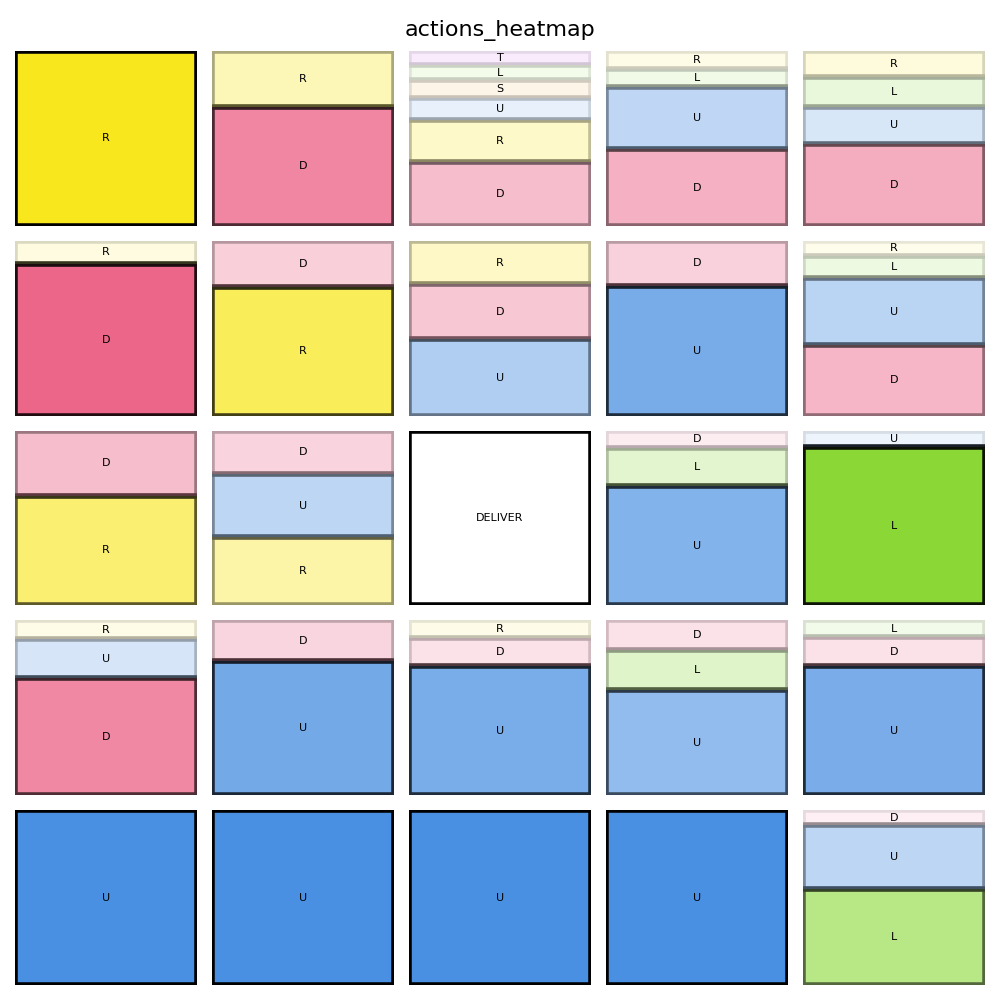
\includegraphics[width=0.8\textwidth]{
    images/data_collection/heatmap_example.png
  }
  \caption{Example of a heatmap generated for a 5x5 map}
  \label{fig:heatmap_example}
\end{figure}

To enhance interpretability, each action is represented using a distinct color:
\begin{itemize}
  \item Green: Left (L)

  \item Yellow: Right (R)

  \item Red: Down (D)

  \item Blue: Up (U)

  \item Purple: Take (T) (picking up a parcel)

  \item Orange: Ship (S) (delivering a parcel)
\end{itemize}
Additionally, the transparency (alpha value) of each color is adjusted based on
the probability of that action, allowing more probable actions to appear more prominently.

A total of 36 test cases have been conducted, and the resulting heatmaps are
stored in the repository under the following directory structure: \begin{verbatim}
../data_and_results/heatmap/heatmaps/MODEL/MAP/GOAL/GOAL_POSITION/
\end{verbatim}
where the last folder contains four files:
\begin{itemize}
  \item \texttt{actions\_heatmap.png}: the rendered heatmap referring to that specific
    test;

  \item \texttt{correctness\_heatmap.png}: the heatmap representing the probability
    of the correct actions that will be discussed in Section \ref{sub:correctness_heatmaps};

  \item \texttt{heatmap.json}: the raw data collected for the heatmap;

  \item \texttt{topX\_values.json}: statistics regarding the \texttt{correctness\_heatmap.png}
    that will be used in the final analysis in Chapter
    \ref{cha:results_discussion}.
\end{itemize}

This organizational structure guarantees that, for each map size, both pickup and
delivery goals are thoroughly tested to cover a wide range of scenarios.
Additionally, in certain cases, we have included other specific goals or prompts
to examine particular behaviors or edge cases of the agent. By incorporating these
varied test configurations, we ensure a comprehensive evaluation of the agent's
performance, which will provide valuable insights for analyzing the results in more
depth.

The location of the goals are varied across different test cases; the rationale
behind choosing ``which tile should be the goal'' will be discussed in Chapter
\ref{cha:results_discussion}.

\subsubsection{Example}

To better understand how to interpret these heatmaps, let us analyze a specific
case. Figure \ref{fig:heatmap_example} presents a heatmap generated for a 5x5 grid,
where the agent's objective is to deliver a parcel at the center of the map.

Consider the cell at coordinates $(2,1)$, which is positioned directly to the left
of the goal. This location is particularly interesting because, being adjacent to
the delivery point, the agent should ideally display a strong preference for
moving Right (R) to complete the task efficiently. The KnowNo framework produced
the following probability distribution for this cell:

\begin{verbatim}
  ...
  {
    "x": 2,
    "y": 1,
    "values": [
      ["R", true, 0.34148147866149986],
      ["U", true, 0.3185527747471083],
      ["D", true, 0.2173149034701972],
      ["T", false, 0.04243503226711094],
      ["L", false, 0.040951236117811166],
      ["S", false, 0.03926457473627248]
    ]
  },
  ...
\end{verbatim}

From this data, we can extract several key observations:
\begin{itemize}
  \item Dominant Actions: The three highest-probability actions at this cell are
    Right (R) with 34.14\%, Up (U) with 31.85\%, and Down (D) with 21.73\%. This
    indicates that while the model slightly favors moving Right, it still considers
    moving Up or Down as viable options;

  \item Discarded Actions: Actions such as Left (L) (4.10\%), Take (T) (4.24\%),
    and Ship (S) (3.93\%) were assigned very low probabilities and subsequently filtered
    out by the KnowNo framework, meaning they were not considered in the final
    action selection process. This suggests that the model appropriately recognizes
    that moving left or attempting to interact with the parcel at this position is
    not optimal;

  \item Probability Normalization: After discarding the low-probability actions,
    the remaining three probabilities were rescaled to sum to 100\%. This renormalization
    ensures that the final action selection is based solely on the most relevant
    choices.
\end{itemize}

This example illustrates how the heatmap helps us diagnose the model’s decision-making
tendencies. Ideally, in this scenario, the probability of moving Right (R)
should be significantly higher, given that it is the only direct path to the goal.
However, the model also considers alternative movements, highlighting potential
limitations in its capabilities.

This example already highlights some potential limitations of the system, particularly
in terms of decision ambiguity when the agent is very near to the goal, which
will be further examined in Chapter \ref{cha:results_discussion}.

\subsection{Correctness Heatmaps}
\label{sub:correctness_heatmaps}

After constructing the action-probability heatmaps, we generate an additional
set of heatmaps that focus on correctness. These correctness heatmaps aim to evaluate
how well the model aligns with the expected optimal behavior by quantifying the probability
assigned to the correct actions at each position in the environment.

To construct these correctness heatmaps, we start determining the set of correct
actions for each cell using a Python script similar to the one in Listing
\ref{lst:correctness_script}. This script systematically analyzes the spatial relationship
between each tile and the designated goal position, identifying which movements
(e.g., U, D, L, R) would bring the agent closer to the goal. The resulting list
of correct actions serves as the reference against which we measure the model's
decision-making accuracy.

\vspace{5mm}
\begin{codewindow}
  [Python Code] \lstset{style=pythonstyle, language=Python, caption={If statements to compute the correct actions for every cell},
  label={lst:correctness_script}} \begin{lstlisting}
for tile in tiles:
    delta_y = goal_y - tile['y']
    delta_x = goal_x - tile['x']
    correct_moves = []
    if delta_x > 0:
        correct_moves.append('D')
    if delta_x < 0:
        correct_moves.append('U')
    if delta_y > 0:
        correct_moves.append('R')
    if delta_y < 0:
        correct_moves.append('L')

    percentage = 0
    for value in tile['values']:
        if value[0] in correct_moves:   # value[0] is the letter
            percentage += value[2]      # value[2] is the probability

    total_percentage = sum([value[2] for value in tile['values']])
    percentage = percentage / total_percentage
\end{lstlisting}
\end{codewindow}
\vspace{5mm}

Once the correct action probabilities have been computed, a second heatmap is
generated. This correctness heatmap visually represents the proportion of probability
assigned to correct actions in each cell. The values are normalized such that
they reflect how much focus the model places on the correct actions relative to
the total probability mass allocated to all retained actions. This allows us to assess
the model's effectiveness in adhering to expected behavior and helps highlight areas
where the agent struggles to make optimal choices.

Figure \ref{fig:correctness_example} illustrates an example correctness heatmap corresponding
to the action probability heatmap shown earlier in Figure \ref{fig:heatmap_example}.

\begin{figure}[ht!]
  \centering
  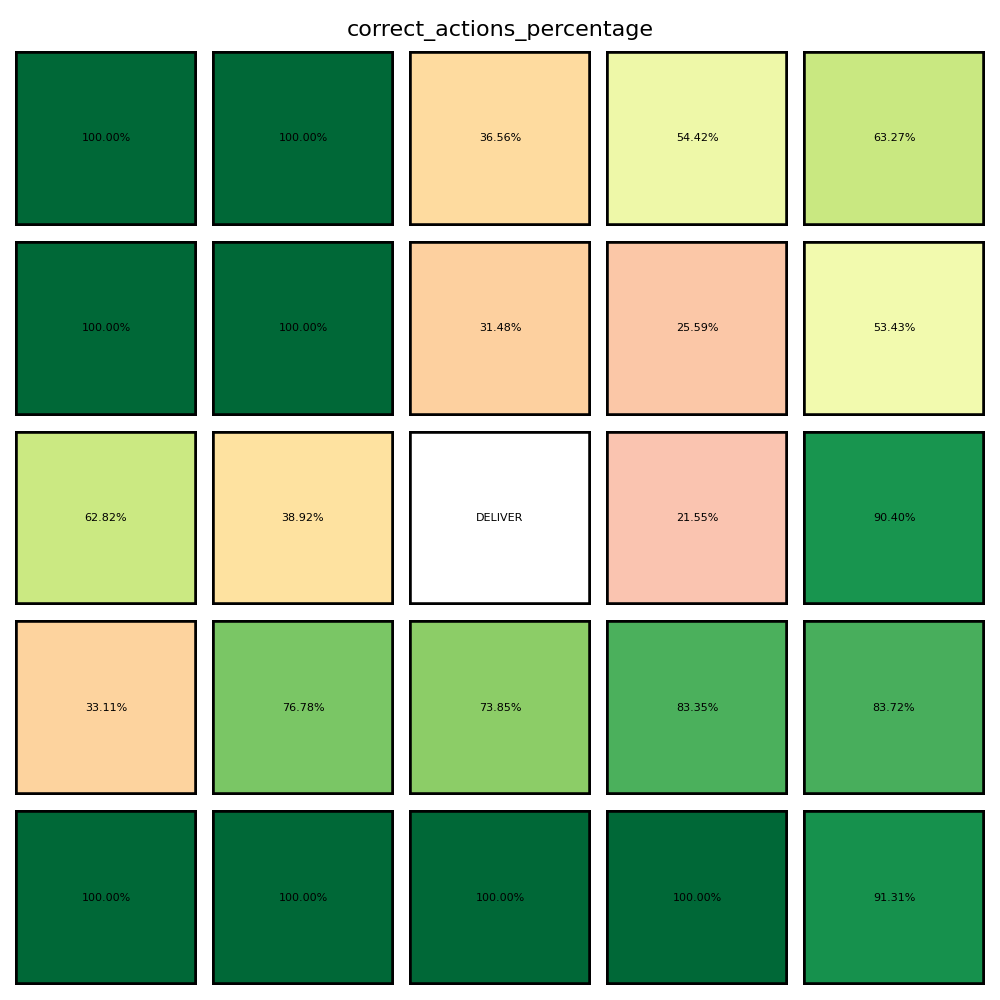
\includegraphics[width=0.8\textwidth]{
    images/data_collection/correctness_example.png
  }
  \caption{Example of a correctness heatmap generated for a 5x5 map}
  \label{fig:correctness_example}
\end{figure}

\subsubsection{Example}

To better understand the significance of the correctness heatmap, let's revisit
the previously analyzed cell at coordinates $(2,1)$, which is located directly to
the left of the goal position in a 5x5 grid.

To compute the correctness probability for this cell, we sum the probability of
the correct action (Right) and normalize it against the total probability mass
assigned to retained actions.

\vspace{5mm}
\begin{codewindow}
  [Text] \lstset{style=promptstyle, language=Prompt, caption={Caption}, label={lst:percentage_compute}}
  \begin{lstlisting}
total_percentage = 0.34148 + 0.31855 + 0.21731 (= 0.87734)
percentage = 0.34148 / total_percentage (= 0.38922)
\end{lstlisting}
\end{codewindow}
\vspace{5mm}

Thus, if the agent selects an action randomly while weighting choices according
to their assigned probabilities (as described in Section \ref{sub:uncertainty_handling}),
in this case it would have a 38.92\% chance of choosing the correct action, as shown
in Listing \ref{lst:percentage_compute}.

This metric provides valuable insight into the model's decision-making tendencies:
while the model recognizes the correct action, it also considers alternative actions
with relatively high probability, indicating uncertainty in its decision-making
process.

By examining correctness heatmaps across different test cases, we can identify patterns
and inconsistencies in the model's behavior. These heatmaps help us pinpoint
areas where the model exhibits high confidence in correct actions and areas
where it is more uncertain or prone to errors.

Some key insights that can be derived from correctness heatmaps include:
\begin{itemize}
  \item High-confidence regions: Cells where the model assigns a near-total
    probability to correct actions indicate strong alignment with expected
    behavior;

  \item Uncertain regions: Areas with distributed probability mass among
    multiple actions suggest indecision, which could stem from ambiguous training
    data or suboptimal model reasoning;

  \item Error-prone zones: Cells where incorrect actions receive a significant
    portion of the probability mass highlight potential weaknesses in the model's
    decision-making.
\end{itemize}
These correctness heatmaps provide a structured way to assess the agent's decision-making
process, offering insights into how well it aligns with expected behavior. By analyzing
these visualizations, we can identify areas where the model exhibits high
confidence in correct actions and regions where it shows uncertainty or
inconsistencies. This analysis will be further explored in Chapter \ref{cha:results_discussion},
where we examine the broader implications of these findings.